% Created by tikzDevice version 0.10.1 on 2016-09-01 16:06:48
% !TEX encoding = UTF-8 Unicode
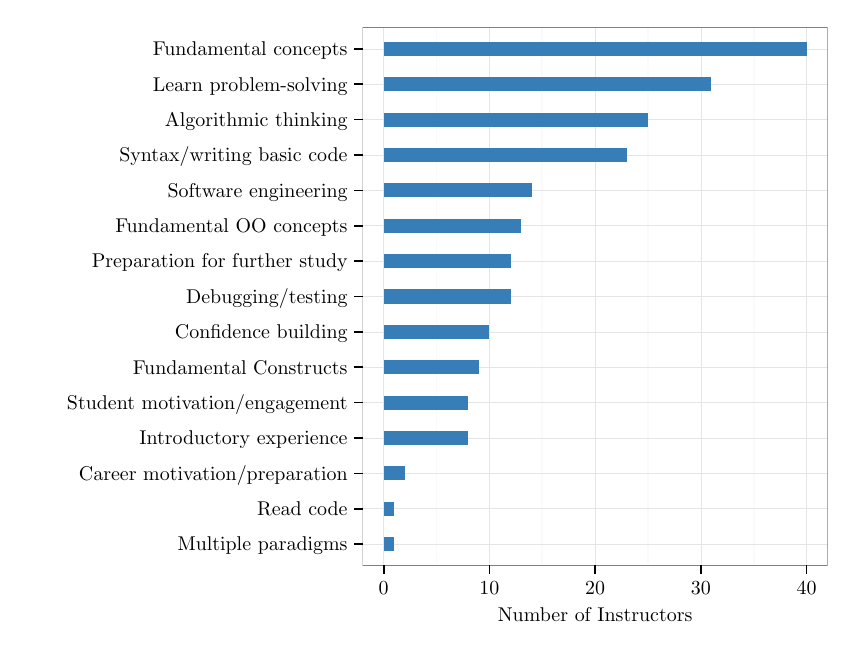
\begin{tikzpicture}[x=1pt,y=1pt]
\definecolor{fillColor}{RGB}{255,255,255}
\path[use as bounding box,fill=fillColor,fill opacity=0.00] (0,0) rectangle (289.08,216.81);
\begin{scope}
\path[clip] (  0.00,  0.00) rectangle (289.08,216.81);
\definecolor{drawColor}{RGB}{255,255,255}
\definecolor{fillColor}{RGB}{255,255,255}

\path[draw=drawColor,line width= 0.6pt,line join=round,line cap=round,fill=fillColor] (  0.00,  0.00) rectangle (289.08,216.81);
\end{scope}
\begin{scope}
\path[clip] (121.00, 22.52) rectangle (289.08,216.81);
\definecolor{fillColor}{RGB}{255,255,255}

\path[fill=fillColor] (121.00, 22.52) rectangle (289.08,216.81);
\definecolor{drawColor}{gray}{0.98}

\path[draw=drawColor,line width= 0.6pt,line join=round] (147.74, 22.52) --
	(147.74,216.81);

\path[draw=drawColor,line width= 0.6pt,line join=round] (185.94, 22.52) --
	(185.94,216.81);

\path[draw=drawColor,line width= 0.6pt,line join=round] (224.14, 22.52) --
	(224.14,216.81);

\path[draw=drawColor,line width= 0.6pt,line join=round] (262.34, 22.52) --
	(262.34,216.81);
\definecolor{drawColor}{gray}{0.90}

\path[draw=drawColor,line width= 0.2pt,line join=round] (121.00, 30.19) --
	(289.08, 30.19);

\path[draw=drawColor,line width= 0.2pt,line join=round] (121.00, 42.97) --
	(289.08, 42.97);

\path[draw=drawColor,line width= 0.2pt,line join=round] (121.00, 55.75) --
	(289.08, 55.75);

\path[draw=drawColor,line width= 0.2pt,line join=round] (121.00, 68.53) --
	(289.08, 68.53);

\path[draw=drawColor,line width= 0.2pt,line join=round] (121.00, 81.32) --
	(289.08, 81.32);

\path[draw=drawColor,line width= 0.2pt,line join=round] (121.00, 94.10) --
	(289.08, 94.10);

\path[draw=drawColor,line width= 0.2pt,line join=round] (121.00,106.88) --
	(289.08,106.88);

\path[draw=drawColor,line width= 0.2pt,line join=round] (121.00,119.66) --
	(289.08,119.66);

\path[draw=drawColor,line width= 0.2pt,line join=round] (121.00,132.45) --
	(289.08,132.45);

\path[draw=drawColor,line width= 0.2pt,line join=round] (121.00,145.23) --
	(289.08,145.23);

\path[draw=drawColor,line width= 0.2pt,line join=round] (121.00,158.01) --
	(289.08,158.01);

\path[draw=drawColor,line width= 0.2pt,line join=round] (121.00,170.79) --
	(289.08,170.79);

\path[draw=drawColor,line width= 0.2pt,line join=round] (121.00,183.58) --
	(289.08,183.58);

\path[draw=drawColor,line width= 0.2pt,line join=round] (121.00,196.36) --
	(289.08,196.36);

\path[draw=drawColor,line width= 0.2pt,line join=round] (121.00,209.14) --
	(289.08,209.14);

\path[draw=drawColor,line width= 0.2pt,line join=round] (128.64, 22.52) --
	(128.64,216.81);

\path[draw=drawColor,line width= 0.2pt,line join=round] (166.84, 22.52) --
	(166.84,216.81);

\path[draw=drawColor,line width= 0.2pt,line join=round] (205.04, 22.52) --
	(205.04,216.81);

\path[draw=drawColor,line width= 0.2pt,line join=round] (243.24, 22.52) --
	(243.24,216.81);

\path[draw=drawColor,line width= 0.2pt,line join=round] (281.44, 22.52) --
	(281.44,216.81);
\definecolor{fillColor}{RGB}{55,126,184}

\path[fill=fillColor] (128.64, 27.63) rectangle (132.46, 32.74);

\path[fill=fillColor] (128.64, 40.41) rectangle (132.46, 45.53);

\path[fill=fillColor] (128.64, 53.20) rectangle (136.28, 58.31);

\path[fill=fillColor] (128.64, 65.98) rectangle (159.20, 71.09);

\path[fill=fillColor] (128.64, 78.76) rectangle (159.20, 83.87);

\path[fill=fillColor] (128.64, 91.54) rectangle (163.02, 96.66);

\path[fill=fillColor] (128.64,104.32) rectangle (166.84,109.44);

\path[fill=fillColor] (128.64,117.11) rectangle (174.48,122.22);

\path[fill=fillColor] (128.64,129.89) rectangle (174.48,135.00);

\path[fill=fillColor] (128.64,142.67) rectangle (178.30,147.79);

\path[fill=fillColor] (128.64,155.45) rectangle (182.12,160.57);

\path[fill=fillColor] (128.64,168.24) rectangle (216.50,173.35);

\path[fill=fillColor] (128.64,181.02) rectangle (224.14,186.13);

\path[fill=fillColor] (128.64,193.80) rectangle (247.06,198.91);

\path[fill=fillColor] (128.64,206.58) rectangle (281.44,211.70);
\definecolor{drawColor}{gray}{0.50}

\path[draw=drawColor,line width= 0.6pt,line join=round,line cap=round] (121.00, 22.52) rectangle (289.08,216.81);
\end{scope}
\begin{scope}
\path[clip] (  0.00,  0.00) rectangle (289.08,216.81);
\definecolor{drawColor}{RGB}{0,0,0}

\node[text=drawColor,anchor=base east,inner sep=0pt, outer sep=0pt, scale=  0.72] at (115.60, 27.71) {Multiple paradigms};

\node[text=drawColor,anchor=base east,inner sep=0pt, outer sep=0pt, scale=  0.72] at (115.60, 40.49) {Read code};

\node[text=drawColor,anchor=base east,inner sep=0pt, outer sep=0pt, scale=  0.72] at (115.60, 53.27) {Career motivation/preparation};

\node[text=drawColor,anchor=base east,inner sep=0pt, outer sep=0pt, scale=  0.72] at (115.60, 66.05) {Introductory experience};

\node[text=drawColor,anchor=base east,inner sep=0pt, outer sep=0pt, scale=  0.72] at (115.60, 78.84) {Student motivation/engagement};

\node[text=drawColor,anchor=base east,inner sep=0pt, outer sep=0pt, scale=  0.72] at (115.60, 91.62) {Fundamental Constructs};

\node[text=drawColor,anchor=base east,inner sep=0pt, outer sep=0pt, scale=  0.72] at (115.60,104.40) {Confidence building};

\node[text=drawColor,anchor=base east,inner sep=0pt, outer sep=0pt, scale=  0.72] at (115.60,117.18) {Debugging/testing};

\node[text=drawColor,anchor=base east,inner sep=0pt, outer sep=0pt, scale=  0.72] at (115.60,129.97) {Preparation for further study};

\node[text=drawColor,anchor=base east,inner sep=0pt, outer sep=0pt, scale=  0.72] at (115.60,142.75) {Fundamental OO concepts};

\node[text=drawColor,anchor=base east,inner sep=0pt, outer sep=0pt, scale=  0.72] at (115.60,155.53) {Software engineering};

\node[text=drawColor,anchor=base east,inner sep=0pt, outer sep=0pt, scale=  0.72] at (115.60,168.31) {Syntax/writing basic code};

\node[text=drawColor,anchor=base east,inner sep=0pt, outer sep=0pt, scale=  0.72] at (115.60,181.10) {Algorithmic thinking};

\node[text=drawColor,anchor=base east,inner sep=0pt, outer sep=0pt, scale=  0.72] at (115.60,193.88) {Learn problem-solving};

\node[text=drawColor,anchor=base east,inner sep=0pt, outer sep=0pt, scale=  0.72] at (115.60,206.66) {Fundamental concepts};
\end{scope}
\begin{scope}
\path[clip] (  0.00,  0.00) rectangle (289.08,216.81);
\definecolor{drawColor}{RGB}{0,0,0}

\path[draw=drawColor,line width= 0.6pt,line join=round] (118.00, 30.19) --
	(121.00, 30.19);

\path[draw=drawColor,line width= 0.6pt,line join=round] (118.00, 42.97) --
	(121.00, 42.97);

\path[draw=drawColor,line width= 0.6pt,line join=round] (118.00, 55.75) --
	(121.00, 55.75);

\path[draw=drawColor,line width= 0.6pt,line join=round] (118.00, 68.53) --
	(121.00, 68.53);

\path[draw=drawColor,line width= 0.6pt,line join=round] (118.00, 81.32) --
	(121.00, 81.32);

\path[draw=drawColor,line width= 0.6pt,line join=round] (118.00, 94.10) --
	(121.00, 94.10);

\path[draw=drawColor,line width= 0.6pt,line join=round] (118.00,106.88) --
	(121.00,106.88);

\path[draw=drawColor,line width= 0.6pt,line join=round] (118.00,119.66) --
	(121.00,119.66);

\path[draw=drawColor,line width= 0.6pt,line join=round] (118.00,132.45) --
	(121.00,132.45);

\path[draw=drawColor,line width= 0.6pt,line join=round] (118.00,145.23) --
	(121.00,145.23);

\path[draw=drawColor,line width= 0.6pt,line join=round] (118.00,158.01) --
	(121.00,158.01);

\path[draw=drawColor,line width= 0.6pt,line join=round] (118.00,170.79) --
	(121.00,170.79);

\path[draw=drawColor,line width= 0.6pt,line join=round] (118.00,183.58) --
	(121.00,183.58);

\path[draw=drawColor,line width= 0.6pt,line join=round] (118.00,196.36) --
	(121.00,196.36);

\path[draw=drawColor,line width= 0.6pt,line join=round] (118.00,209.14) --
	(121.00,209.14);
\end{scope}
\begin{scope}
\path[clip] (  0.00,  0.00) rectangle (289.08,216.81);
\definecolor{drawColor}{RGB}{0,0,0}

\path[draw=drawColor,line width= 0.6pt,line join=round] (128.64, 19.52) --
	(128.64, 22.52);

\path[draw=drawColor,line width= 0.6pt,line join=round] (166.84, 19.52) --
	(166.84, 22.52);

\path[draw=drawColor,line width= 0.6pt,line join=round] (205.04, 19.52) --
	(205.04, 22.52);

\path[draw=drawColor,line width= 0.6pt,line join=round] (243.24, 19.52) --
	(243.24, 22.52);

\path[draw=drawColor,line width= 0.6pt,line join=round] (281.44, 19.52) --
	(281.44, 22.52);
\end{scope}
\begin{scope}
\path[clip] (  0.00,  0.00) rectangle (289.08,216.81);
\definecolor{drawColor}{RGB}{0,0,0}

\node[text=drawColor,anchor=base,inner sep=0pt, outer sep=0pt, scale=  0.72] at (128.64, 12.16) {0};

\node[text=drawColor,anchor=base,inner sep=0pt, outer sep=0pt, scale=  0.72] at (166.84, 12.16) {10};

\node[text=drawColor,anchor=base,inner sep=0pt, outer sep=0pt, scale=  0.72] at (205.04, 12.16) {20};

\node[text=drawColor,anchor=base,inner sep=0pt, outer sep=0pt, scale=  0.72] at (243.24, 12.16) {30};

\node[text=drawColor,anchor=base,inner sep=0pt, outer sep=0pt, scale=  0.72] at (281.44, 12.16) {40};
\end{scope}
\begin{scope}
\path[clip] (  0.00,  0.00) rectangle (289.08,216.81);
\definecolor{drawColor}{RGB}{0,0,0}

\node[text=drawColor,anchor=base,inner sep=0pt, outer sep=0pt, scale=  0.72] at (205.04,  2.40) {Number of Instructors};
\end{scope}
\end{tikzpicture}
